\begin{figure}[t]
    \centering

    % ---------------------------------------------------------
    % (a)
    % ---------------------------------------------------------
    \begin{subfigure}[t]{0.47\textwidth}
        \centering

        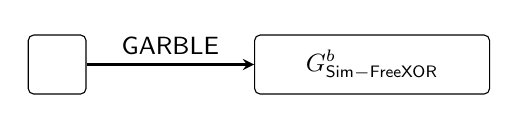
\begin{tikzpicture}[
            font=\small,
            >=stealth,
            adversary/.style={
                draw,
                rounded corners=2pt,
                minimum width=5mm,
                text width=5mm,
                minimum height=0.75cm,
                align=center
            },
            box/.style={
                draw,
                rounded corners=2pt,
                minimum height=0.75cm,
                align=center
            },
            arrow/.style={->, thick}
        ]

            \node[adversary] (A) at (-1,0) {$\adv$};
            \node[box, text width=2.75cm, minimum width=2.75cm] (G) at (3,0) {$G^{b}_\mathsf{Sim\text{-}FreeXOR}$};

            \draw[arrow] (A) -- node[above] {$\mathsf{GARBLE}$} (G);

        \end{tikzpicture}

        \caption{Adversary $\adv$ calls oracle $\mathsf{GARBLE}$ of Sim-FreeXOR Game}
        \label{fig:gamehopping-a}
    \end{subfigure}
    \hfill
    % ---------------------------------------------------------
    % (b)
    % ---------------------------------------------------------
    \begin{subfigure}[t]{0.47\textwidth}
        \centering

        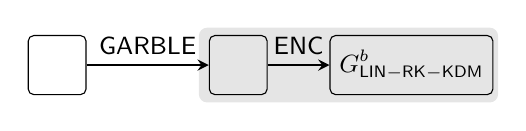
\begin{tikzpicture}[
            font=\small,
            >=stealth,
            adversary/.style={
                draw,
                rounded corners=2pt,
                minimum width=5mm,
                text width=5mm,
                minimum height=0.75cm,
                align=center
            },
            reduction/.style={
                draw,
                rounded corners=2pt,
                minimum width=5mm,
                text width=5mm,
                minimum height=0.75cm,
                align=center
            },
            box/.style={
                draw,
                rounded corners=2pt,
                minimum width=1.3cm,
                minimum height=0.75cm,
                align=center
            },
            arrow/.style={->, thick},
            shade/.style={
                fill=gray!20,
                draw=none,
                rounded corners=3pt
            }
        ]

            % Shading
            \node[
                shade,
                minimum width=3.8cm,
                minimum height=0.95cm
            ] at (2.7,0) {};

            \node[adversary] (A) at (-1,0) {$\adv$};
            \node[reduction] (R) at (1.3,0) {$\rdv$};
            \node[box] (G) at (3.5,0) {$G^{b}_{\mathsf{LIN-RK-KDM}}$};

            \draw[arrow] (A) -- node[above] {$\mathsf{GARBLE}$} (R);
            \draw[arrow] (R) -- node[above] {$\mathsf{ENC}$} (G);

            
        \end{tikzpicture}

        \caption{Sim-FreeXOR game $\codeequiv$ $\rdv\to$ {LIN-RK-KDM} game }
        \label{fig:gamehopping-b}
    \end{subfigure}

    \vspace{1em}

    % ---------------------------------------------------------
    % (c)
    % ---------------------------------------------------------
    \begin{subfigure}[t]{0.47\textwidth}
        \centering

        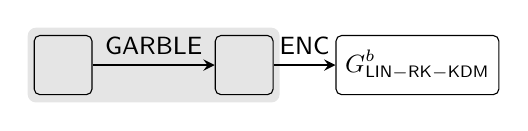
\begin{tikzpicture}[
            font=\small,
            >=stealth,
            adversary/.style={
                draw,
                rounded corners=2pt,
                minimum width=5mm,
                text width=5mm,
                minimum height=0.75cm,
                align=center
            },
            reduction/.style={
                draw,
                rounded corners=2pt,
                minimum width=5mm,
                text width=5mm,
                minimum height=0.75cm,
                align=center
            },
            box/.style={
                draw,
                rounded corners=2pt,
                minimum width=1.3cm,
                minimum height=0.75cm,
                align=center
            },
            arrow/.style={->, thick},
            shade/.style={
                fill=gray!20,
                draw=none,
                rounded corners=3pt
            }
        ]

            % Shading
            \node[
                shade,
                minimum width=3.2cm,
                minimum height=0.95cm
            ] at (0.15,0) {};

            \node[adversary] (A) at (-1,0) {$\adv$};
            \node[reduction] (R) at (1.3,0) {$\rdv$};
            \node[box] (G) at (3.5,0) {$G^{b}_{\mathsf{LIN-RK-KDM}}$};

            \draw[arrow] (A) -- node[above] {$\mathsf{GARBLE}$} (R);
            \draw[arrow] (R) -- node[above] {$\mathsf{ENC}$} (G);

            
        \end{tikzpicture}

        \caption{Associativity allows us to compose $\adv\to\rdv$}
        \label{fig:gamehopping-c}
    \end{subfigure}
    \hfill
    % ---------------------------------------------------------
    % (d)
    % ---------------------------------------------------------
    \begin{subfigure}[t]{0.47\textwidth}
        \centering

        
        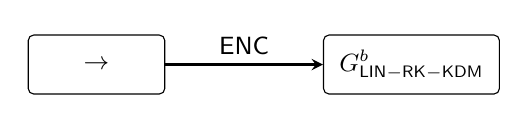
\begin{tikzpicture}[
            font=\small,
            >=stealth,
            box/.style={
                draw,
                rounded corners=2pt,
                minimum width=2cm,
                text width=2cm,
                minimum height=0.75cm,
                align=center
            },
            adversary/.style={
                draw,
                rounded corners=2pt,
                minimum height=0.75cm,
                align=center
            },
            arrow/.style={->, thick}
        ]

            \node[adversary, text width=1.5cm, minimum width=1.5cm] (A) at (-1,0) {$\adv\to\rdv$};
            \node[box] (G) at (3,0) {$G^{b}_{\mathsf{LIN-RK-KDM}}$};

            \draw[arrow] (A) -- node[above] {$\mathsf{ENC}$} (G);

        \end{tikzpicture}

        \caption{The composed adversary $\adv\to\rdv$ calls oracle $\mathsf{ENC}$ of the {LIN-RK-KDM} game}
        \label{fig:gamehopping-d}
    \end{subfigure}

    \caption{A visualization of the adversary transformation in the proof in Section \ref{subsec:andgate}}
    \label{fig:game-reduction}

\end{figure}